\documentclass[twoside,10pt,a4paper]{article}
\usepackage[utf8]{inputenc}
\usepackage[english]{babel}
\usepackage{amsmath}
\usepackage{amsfonts}
\usepackage{amssymb}
\usepackage{graphicx}

\usepackage[left=2cm,right=2cm,top=2cm,bottom=3cm]{geometry}
\usepackage{fancyvrb}
\usepackage{listings}
\usepackage{xparse}
\usepackage{tikz} % ajout de dessins LaTeX
\usepackage{graphicx}
\usepackage{float}  % alignement des figures
\usepackage{fancyhdr}
\usepackage{enumitem}
\usepackage{verbatim}
\usepackage{xcolor}
\usepackage{cancel}

\usepackage{caption}
\usepackage{subcaption}

\pagestyle{fancy} %fancyhdr
	\fancyhf{} %fancyhdr
	\renewcommand{\sectionmark}[1]{\markboth{#1}{}}
	\fancyhead[R]{NLDCI Set 4 Solutions} %INSERT TITLE HERE FOR fancyhdr
	\fancyhead[L]{\nouppercase{\leftmark}} %fancyhdr
	\cfoot{\thepage} %fancyhdr
	\setlength{\headheight}{35pt}
	\setlength{\parindent}{0pt}

\begin{titlepage}
\title{\huge \textbf{Nonlinear Dynamics \& Chaos I \\ \Large Exercice Set 4 Solutions}}	%TITLE
\author{ }		%AUTHOR
\date{ }	%DATE

\end{titlepage}

	\definecolor{MyBlue}{HTML}{4A90E2}
	\definecolor{MyRed}{HTML}{D0021B}
	\definecolor{MyGreen}{HTML}{7ED321} % Same color use in Mathcha


\begin{document}

\maketitle

\section*{Question 1}
Consider the discrete dynamical system
\begin{align*}
	x_{n+1} &= Ax_n + f(x_n, y_n), \\
	y_{n+1} &= By_n + g(x_n, y_n),
\end{align*}
where $x_n \in \mathbb{R}^c$, $y_n \in \mathbb{R}^d$, $A \in \mathbb{R}^{c \times c}$, $B \in \mathbb{R}^{d \times d}$; $f$ and $g$ are $C^r$ functions with no linear terms. Assume that all eigenvalues of $A$ have modulus one, and none of the eigenvalues of $B$ have modulus one. Then the linearized system at the origin admits a center subspace $E^c$ aligned with the $x$-coordinate plane.

\begin{enumerate}[label=(\alph*)]
	\item Derive a general algebraic equation for the center manifold $W^c$, which is known to exist by a theorem analogous to the center manifold theorem for continuous dynamical systems.
	\item Find a cubic order approximation for the center manifold of the discrete system
	\begin{align*}
		x_{n+1} &= x_n + x_ny_n, \\
		y_{n+1} &= \lambda y_n - x_n^2,
	\end{align*}
	where $\lambda \in (0,1).$
	\item Reduce the dynamics to the center manifold and determine the stability of the origin. Verify your results by a numerical simulation of a few initial conditions near the origin.
\end{enumerate}

\section*{Solution 1}
\begin{enumerate}[label=(\alph*)]
\item Let the graph of the center manifold near the origin be given by $y = h(x), \; h:\mathbb{R}^c \rightarrow \mathbb{R}^d$
\begin{figure}[H]
	\centering
	\includegraphics[scale=0.9]{Graphics/S01D01.pdf}
\end{figure}
By the invariance of the center manifold we have $y_n = h(x_n)$ for all $n$.

\begin{equation*}
	y_{n+1} = h(x_{n+1})
\end{equation*}
But
\begin{align*}
	y_{n+1} &= By_n + g(x_n, y_n) \\
	&= Bh(x_n) + g(x_n, h(x_n))
\end{align*}
and
\begin{align*}
	x_{n+1} &= Ax_n + f(x_n, y_n) \\
	&= Ax_n + f(x_n, h(x_n))
\end{align*}
Hence
\begin{equation*}
	Bh(x_n) + g(x_n, h(x_n)) = h[Ax_n + f(x_n, h(x_n))]
\end{equation*}
Therefore, the function $h:\mathbb{R}^c \rightarrow \mathbb{R}^d$ satisfies

\begin{equation}\label{S04E011}\boxed{
		Bh(x) + g(x, h(x)) = h[Ax + f(x, h(x))]
	}
\end{equation}


\item Here, $[A] = [1],\; [B] = [\lambda], \; f(x_n,y_n) = x_ny_n$ and $g(x_n, y_n)=-x_n^2$.

Since $h$ passes through the origin and it is tangent to the $x$-axis, we have $h(0)=0$ and $h'(0)=0$. (Note that here $c=d=1 \Rightarrow h:\mathbb{R} \rightarrow \mathbb{R}$).

Therefore, the Taylor expansion of $h$ around $x=0$ has the form
\begin{equation}\label{S04E012}
	h(x) = ax^2 + bx^3 + \mathcal{O}(x^4)
\end{equation}
Equation (\ref{S04E011}) for the current system is: $\lambda h(x) - x^2 = h(x + xh(x))$.

Substituting (\ref{S04E012}) in this equation we get
\begin{align*}
	\lambda(ax^2 + bx^3 + \mathcal{O}(x^4)) - x^2 &= h[x + ax^3 + \mathcal{O}(x^4)] \\
	&= a(x + ax^3 + \mathcal{O}(x^4))^2 + b(x + ax^3 + \mathcal{O}(x^4))^3 + \cdots
\end{align*}
\begin{equation*}
	\Longrightarrow (\lambda a - 1)x^2 + \lambda b x^3 + \mathcal{O}(x^4) = ax^2 + bx^3 + \mathcal{O}(x^4)
\end{equation*}
Matching the exponents from both sides we obtain:
\begin{align*}
	\lambda a - 1 = a &\Longrightarrow a = \frac{1}{\lambda - 1} \\
	\lambda b = b &\Longrightarrow b = 0
\end{align*}
and finally
\begin{equation*}
	\boxed{
		h(x) = \frac{1}{\lambda - 1}x^2 + \mathcal{O}(x^4)	
	}
\end{equation*}


\item The center manifold near the origin satisfies $h(x) \approx \frac{1}{\lambda - 1}x^2$.
Hence, the dynamics on the center manifold satisfy

\begin{align}
	x_{n+1} &= x_n + \frac{1}{\lambda - 1}x_n^3 \nonumber \\
	\Longrightarrow x_{n+1} &= x_n \left( 1 + \frac{1}{\lambda - 1}x_n^2 \right) \label{S04E013}
\end{align}
In the following, we show that the fixed point $x=0$ of (\ref{S04E013}) is asymptotically stable. 

First let $x_0 \in \mathbb{R}$ with $|x_0|>0$ small enough be an initial condition. Then if
\begin{equation}\label{S04E014}
	\left\vert 1 + \frac{1}{\lambda - 1}x_0^2 \right\vert < 1
\end{equation}
we have
\begin{equation*}
	|x_1| \leq \left\vert x_0 \left( 1 + \frac{1}{\lambda - 1}x_0^2 \right) \right\vert < |x_0|
\end{equation*}
Inequality (\ref{S04E014}) holds if and only if $|x_1| < |x_0| < \sqrt{2(1-\lambda)}$. That is for any $x_0$ with $|x_0|<\sqrt{2(1-\lambda)}$ we have $|x_1| < |x_0| < \sqrt{2(1-\lambda)}$.

For such initial conditions, we have (by induction):
\begin{equation}\label{S04E015}
	\cdots < |x_{n+1}| < |x_n| < \cdots < |x_1| < |x_0| < \sqrt{2(1-\lambda)}
\end{equation}
This proves that the stability of the fixed point $x=0$. To prove asymptotic stability, we need
\begin{equation*}
	\lim_{n \rightarrow \infty} x_n = 0
\end{equation*}

Note that the sequence $\{|x_n|\}$ is a decreasing (due to (\ref{S04E015})) sequence that is bounded from below $(|x_n| \geq 0)$. Therefore, it must have a limit:
\begin{equation*}
	\lim_{n \rightarrow \infty} |x_n| = \alpha
\end{equation*}

This limit, in general, doesn't have to be zero. But taking the limit $n \rightarrow \infty$ in equation (\ref{S04E013}) we get
\begin{equation*}
	\lim_{n \rightarrow \infty} |x_{n+1}| = \lim_{n \rightarrow \infty}
	|x_n| \left( 1 + \frac{1}{\lambda - 1} \lim_{n \rightarrow \infty} |x_n|^2 \right)
\end{equation*}
\begin{equation*}
	\alpha = \alpha \left( 1 + \frac{1}{\lambda - 1} \alpha^2 \right) \Longrightarrow \alpha = 0 \Longrightarrow \lim_{n \rightarrow \infty} x_n = 0
\end{equation*}
Therefore the fixed point is asymptotically stable.
\vspace{15 pt}
The following figure shows the iterations of the map for four initial conditions marked by square symbols. The higher iterations are marked by dots. The black curve marks the approximate center manifold:
\begin{equation*}
	y = \frac{1}{\lambda - 1}x^2
\end{equation*}


\begin{Verbatim}[numbers = left]
	%% Initiation

	close all
	clear all
	clc

	%% Main

	lambda = 0.5;
	x = linspace(-0.5, 0.5, 50);
	
	y = x.^2/(lambda - 1);
	
	figure;
	plot(x,y)
	
	maxIter = 1000;
	
	xn = zeros(maxIter + 1, 1);
	yn = zeros(maxIter + 1, 1);
	
	% Initial Conditions
	
	xn1(1) = -0.1;
	yn1(1) = 0.1;
	
	xn2(1) = 0.1;
	yn2(1) = 0.1;
	
	xn3(1) = -0.25;
	yn3(1) = 0.25;
	
	xn4(1) = 0.25;
	yn4(1) = 0.25;
	
	% Interations
	
	for j = 1:maxIter
	    [xn1(j+1), yn1(j+1)] = map(xn1(j), yn1(j), lambda);
	end
	
	for j = 1:maxIter
	    [xn2(j+1), yn2(j+1)] = map(xn2(j), yn2(j), lambda);
	end
	
	for j = 1:maxIter
	    [xn3(j+1), yn3(j+1)] = map(xn3(j), yn3(j), lambda);
	end
	
	for j = 1:maxIter
	    [xn4(j+1), yn4(j+1)] = map(xn4(j), yn4(j), lambda);
	end
	
	hold on
	plot(xn1, yn1, '*r')
	plot(xn2, yn2, '*r')
	plot(xn3, yn3, '*g')
	plot(xn4, yn4, '*g')
	xlabel('$x$','interpreter','latex')
	ylabel('$y$','interpreter','latex')
	grid on
		
	%% Function
	
	function [x1, y1] = map(x0, y0, lambda)
	    x1 = x0 + x0 * y0;
	    y1 = lambda * y0 - x0^2;
	end
\end{Verbatim}

\newpage

This MATLAB code gives the following figure:
\begin{figure}[H]
	\centering
	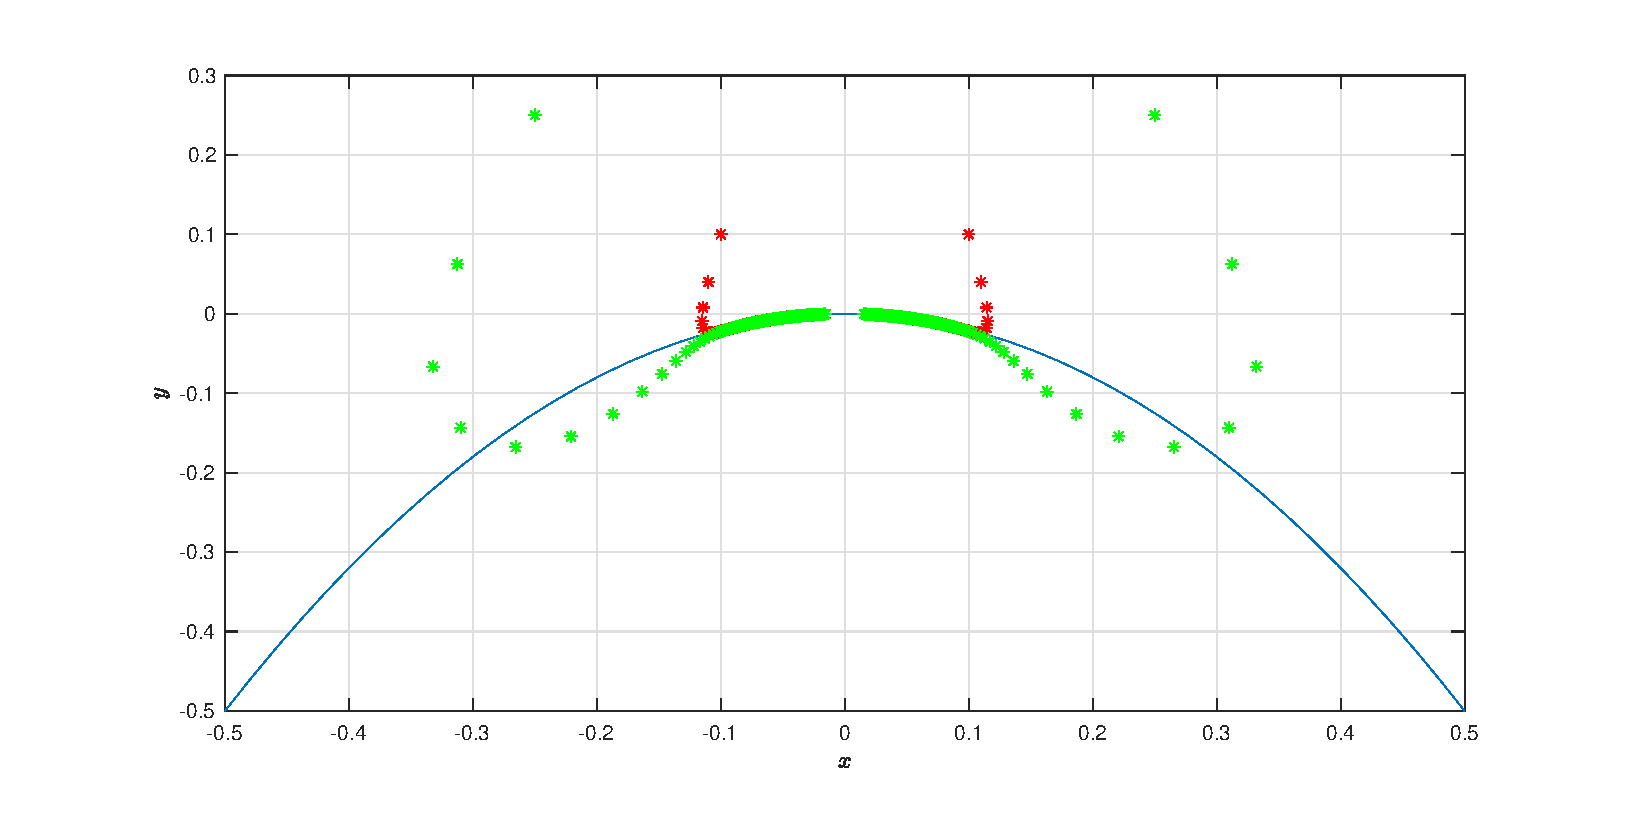
\includegraphics[scale=0.5]{Graphics/S01D02.eps}
\end{figure}

\end{enumerate}

\newpage

\section*{Question 2}
Construct a cubic-order local approximation for the unstable manifold of the hyperbolic fixed point of the pendulum equation
\begin{equation*}
	\ddot{x} + \sin(x) = 0.
\end{equation*}

\section*{Solution 2}
\begin{figure}[H]
	\centering
	\includegraphics[scale=0.9]{Graphics/S02D01.pdf}
\end{figure}
Let $x_1 = x$ and $x_2 = \dot{x}$. Then:
\begin{equation*}
	\begin{cases}
		\dot{x}_1 = x_2 \\
		\dot{x}_2 = -\sin(x_1)
	\end{cases}
\end{equation*}
By linearization, one can show that the fixed point $(\pi, 0)$ is an unstable hyperbolic fixed point with stable and unstable linear subspaces spanned by $\begin{pmatrix} 1 \\ 1 \end{pmatrix}$ and $\begin{pmatrix} 1 \\ -1 \end{pmatrix}$, respectively:
\begin{figure}[H]
	\centering
	\includegraphics[scale=0.9]{Graphics/S02D02.pdf}
\end{figure}
For convenience, we shift the origin by the transformation $\xi_1 = x_1 - \pi$ and $\xi_2 = x_2$ such that in $(\xi_1 , \xi_2)$ the origin is the hyperbolic fixed point.

In this coordinate system, the dynamical system becomes:
\begin{equation*}
	\begin{cases}
		\dot{\xi}_1 = \xi_2 \\
		\dot{\xi}_2 = \sin(\xi_1)
	\end{cases} \qquad (\text{since } -\sin(x_1) = -\sin(\xi_1 + \pi) = \sin(\xi_1))
\end{equation*}
The unstable manifold passing through the origin is a graph over $\xi_1$ and tangent to $E^U$.
\begin{figure}[H]
	\centering
	\includegraphics[scale=0.9]{Graphics/S02D03.pdf}
\end{figure}
If this graph is given by $\xi_2 = h(\xi_1)$, the Taylor expansion of $h$ looks like:
\begin{equation*}
	h(\xi_1) = \underbrace{0}_{h(0)=0} + \underbrace{\xi_1}_{h'(0)=1} + a\xi_1^2 + b\xi_1^3 + \mathcal{O}(\xi_1^4)
\end{equation*}
By invariance of the unstable manifold we have $\dot{\xi}_2 = h'(\xi_1) \dot{\xi}_1$

Therefore,
\begin{equation*}
	\sin(\xi_1) = (1 + 2a\xi_1 + 3b\xi_1^2 + \mathcal{O}(3))(\xi_1 + a\xi_1^2 + b\xi_1^3 + \mathcal{O}(4))
\end{equation*}
The Taylor expansion of $\sin(\xi_1)$ around $\xi_1=0$ reads
\begin{equation*}
	\sin(\xi_1) = \xi_1 - \frac{1}{6}\xi_1^3 + \mathcal{O}(\xi_1^5)
\end{equation*}
Matching exponents we get $a = 0$ and $b = -\frac{1}{24}$.

Therefore, the graph of unstable manifold satisfies:
\begin{equation*}
	\xi_2 = \xi_1 - \frac{1}{24}\xi_1^3 + \mathcal{O}(\xi_1^4)
\end{equation*}
or
\begin{equation*}\boxed{
	x_2 = x_1 - \pi -\frac{1}{24}(x_1 - \pi)^3 + \mathcal{O}(|x_1 - \pi|^4)
}\end{equation*}

\newpage

\section*{Solution 3}
Consider the discrete dynamical system
\begin{equation*}
	\begin{cases}
		x_{n+1} = x_n + x_ny_n \\
		y_{n+1} = \frac{1}{2}y_n - x_n^2
	\end{cases}
\end{equation*}
Let $h:(-\varepsilon, \varepsilon) \longrightarrow \mathbb{R}$ be the local graph of the \underline{center manifold} around $(0,0)$. $(0 < \varepsilon \ll 1)$. Find the expressions that $h$ satisfies.

\begin{enumerate}[label=(\alph*)]
	\item $ \displaystyle h(x + h(x)) - \frac{1}{2}h(x) = x^2 $
	\item $ \displaystyle h(x + h(x)) - \frac{1}{2}h(x) = -x^2 $
	\item $ \displaystyle h(x + xh(x)) - \frac{1}{2}h(x) = x^2 $
	{\color{MyRed}\item $ \displaystyle h(x + xh(x)) - \frac{1}{2}h(x) = -x^2 $}
\end{enumerate}

\section*{Solution 4}
Consider the following dynamical system
\begin{equation*}
	\begin{cases}
		\dot{x} = xy \\
		\dot{y} = -y + x^2
	\end{cases}
\end{equation*}
Which expression describes the reduced dynamics on the center manifold?

\begin{enumerate}[label=(\alph*)]
	{\color{MyRed}\item $ \dot{x} = x^3(1 - 2x^2) + \mathcal{O}(x^5) $}
	\item $ \dot{y} = y^3(1 - 2y^2) + \mathcal{O}(y^5) $
	\item $ \dot{x} = x^3(1 + 2x^2) + \mathcal{O}(x^5) $
	\item $ \dot{y} = y^3(1 + 2y^2) + \mathcal{O}(y^5) $
\end{enumerate}

\section*{Solution 5}
Consider the following dynamical system
\begin{equation*}
	\begin{cases}
		\dot{x} = -x^3 \\
		\dot{y} = -y
	\end{cases}
\end{equation*}
Let $y = h(x)$ be the graph of the center manifold of $(0,0)$. Which of the following expressions is accurate ?

\textit{Hint}: $ \displaystyle \frac{dy}{dx} = \frac{\dot{y}}{\dot{x}} = \frac{y}{x^3} $

\begin{enumerate}[label=(\alph*)]
	\item The dynamical system has a unique center manifold with $ \displaystyle h(x) = e^{-\frac{1}{2x^2}} $
	\item The dynamical system has a unique center manifold with $ \displaystyle h(x) = e^{-\frac{1}{x^2}} $
	{\color{MyRed}\item The dynamical system has infinitely many center manifolds with $ \displaystyle h(x) = \begin{cases}
		ae^{-\frac{1}{2x^2}} & x < 0 \\
		0 & x = 0 \\
		be^{-\frac{1}{2x^2}} & x > 0
	\end{cases} \;\; \forall a,b \in \mathbb{R}$}
	\item The dynamical system has infinitely many center manifolds with $ \displaystyle h(x) = \begin{cases}
		ae^{-\frac{1}{x^2}} & x < 0 \\
		0 & x = 0 \\
		be^{-\frac{1}{x^2}} & x > 0
	\end{cases} \;\;  \forall a,b \in \mathbb{R}$
\end{enumerate}

{\color{MyRed}
\begin{equation*}
	\int_{y_0}^y \frac{dy}{y} = \int_{x_0}^x \frac{dx}{x^3} \Longrightarrow y = Ce^{-\frac{1}{2x^2}}
\end{equation*}

All such invariant curves are center manifold candidates as their derivative vanishes at the origin.
}

\section*{Solution 6}
The phase portrait of four planar dynamical systems are shown below. In which case is the origin \underline{not} Lyapunov stable?

\begin{enumerate}[label=(\alph*)]
	\item \includegraphics[scale=0.8]{Graphics/MCQ1_figures/Q17D01.pdf}
	\item \includegraphics[scale=0.8]{Graphics/MCQ1_figures/Q17D02.pdf}
	\item \includegraphics[scale=0.8]{Graphics/MCQ1_figures/Q17D03.pdf}
	{\color{MyRed}\item 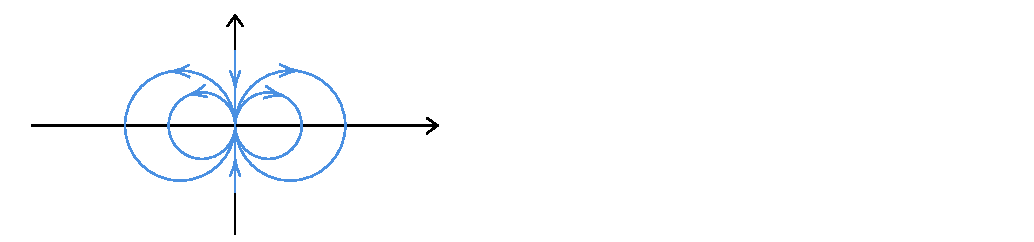
\includegraphics[scale=0.8]{Graphics/MCQ1_figures/Q17D04.pdf}}
\end{enumerate}

\section*{Solution 7}
Consider the dynamical system below
\begin{equation*}
	\dot{x} = |x|^2 (Ax + f(x))
\end{equation*}
where , $x \in \mathbb{R}^n, \; f \in C^1, \; A \in \mathbb{R}^{n \times n}, \; f = \mathcal{O}(|x|^2)$ and the matrix $A$ has precisely one pair of purely imaginary eigenvalues, and $(n - 2)$ eigenvalues with negative real parts.

Which of the following statements are true?

\begin{enumerate}[label=(\alph*)]
	\item The origin $x = 0$ is unstable.
	\item $ \dim(W^c(0)) = 2 $
	{\color{MyRed}\item$ \dim(W^c(0)) = n $}
	\item None of the above
\end{enumerate}


\end{document}